\documentclass{matmex-diploma-custom}
\usepackage{amsfonts}

\begin{document}
\filltitle{ru}{
  chair = {Кафедра Системного Программирования},
  title = {Построение генетических карт по неполным и зашумленным данным},
  type = {diploma},
  position = {студентки},
  group = 545,
  author = {Крамар Алина Сергеевна},
  supervisorPosition = {к.\,ф.-м.\,н., доцент},
  supervisor = {Сысоев С.\,С.},
  reviewerPosition = {науч. сотрудник.},
  reviewer = {Добрынин П.В.},
  chairHeadPosition = {д.\,ф.-м.\,н., профессор},
  chairHead = {Терехов А.\,Н.},
  university = {Санкт-Петербургский Государственный Университет},
  faculty = {Математико-механический факультет},
  city = {Санкт-Петербург},
  year = {2014}
}
\filltitle{en}{
  chair = {Department of Software Engineering},
  title = {Genetic linkage mapping based on incomplete and noisy data},
  author = {Alina Kramar},
  supervisorPosition = {associate professor},
  supervisor = {Sergey Sysoev},
  reviewerPosition = {research associate},
  reviewer = {Pavel Dobrynin},
  chairHeadPosition = {professor},
  university = {Saint Petersburg State University},
  chairHead = {Andrey Terekhov}
}
\maketitle \tableofcontents
\section*{Введение}

Краткая медицинская энциклопедия \cite{petrovsky1989} даёт следующее
определение слову “генетика”: наука о наследственности и изменчивости
организма. Согласно законам наследования все основные признаки и
свойства любых организмов определяются и контролируются единицами
наследственной информации - генами, локализованными в специфических
структурах клетки - хромосомах
\cite{griffiths2005introduction,griffiths2000introduction}. В связи с
этим, основной задачей генетики является на основе первичной структуры
биополимеров (молекул ДНК или РНК) определить фенотип особи, механизмы
наследования тех или иных признаков и т.п. Получение информации о
первичной структуре ДНК называется секвенированием \cite{cito1994}. К
сожалению, современные методы секвенирования не в состоянии
предоставить информацию о полной нуклеатидной последовательности в
рамках конкретной хромосомы \cite{molecular}. Сама по себе
нуклеатидная последовательность не содержит прямой информации о
происхождении того или иного однозначно идентифицируемого участка
(маркера), и становится затруднительным определить, от какого предка
был унаследован тот или иной признак. Для определения шаблонов
наследования и выявления его принципов предназначены генетические
карты хромосом \cite{morgan1922mechanism}.

Генетическая карта - это схема или порядок расположения маркеров на
хромосоме (здесь и далее подразумевается структурный маркер,
т.е. маркер, имеющий отличимое нуклеатидное представление, которое
позволяет его идентифицировать) и генов. Зачастую, наличие генов не
так важно, как наличие маркеров, потому что гены имеют свойство
наследоваться не полностью \cite{schiller2010genome}. Идея создать
генные карты принадлежит Томасу Моргану, внёсшему неоспоримый вклад в
теорию наследственности. Идея была основана на явлении сцепленного
наследования генов. Из-за мейотического кроссинговера, который делает
невозможным полностью скоррелированное наседование и влияет на
расхождение сцепленных генов по разным гаметам, появилось
предположение о связи физического расстояния между маркерами и их
взаимодействии при наследовании \cite{creighton1931correlation}. Это
предположение оправдалось, и в 1913 году ученик Моргана Альфред
Стёртевант построил первую генетическую карту на основе данных
Drosophila melanogaster
\cite{goldhor1962genetics,sturtevant1939introduction}.

Кроссинговер на этапе мейоза вносит возмущение в сцепленное
наследование \cite{creighton1931correlation}, и чем чаще он
проявляется, тем чаще наблюдается отклонение от сцеплений. Физическое
расстояние между парой генов прямо пропорционально вероятности
кроссинговера, что позволяет однозначно расположить маркеры на
молекуле \cite{sturtevant1939introduction}. Генетическое расстояние не
трудно перевести в физическое, но чаще всего в этом нет необходимости,
так как для механизма наследования существенен порядок
\cite{hartl2011genetics, malacinski2005essentials}. Единицей измерения
расстояния является 1 сантиморган. Стоит упомянуть, что задача
построения генетической карты хромосомы имеет смысл для диплоидных
особей и лучше решается, когда исследуемые особи находятся в родстве
\cite{meiosi}. Задача так же решается проще на семействах особей,
которые размножаются c большой скоростью (больше данных), поэтому
большее количество карт на данный момент имеют хромосомы дрозофил,
кошек, мелких грызунов и насекомых \cite{mcpeek1996introduction}. Нас
же интересуют генетические карты человека, так как эти карты являются
единственным способом проведения генетического анализа на наличие и
предрасположенность особи к тяжёлым наследственным заболеваниям. С
помощью генетического анализа можно выявлять болезнь Альцгеймера
\cite{schellenberg1992genetic}, гемофилию \cite{oberle1985genetic},
хорею Хаттингтона \cite{anderson2004polymorphic} и т.п.

Современные средства генетического картирования позволяют построить
карту по форматированному файлу родословной \cite{lander1987mapmaker,
  crimap, lmmap}. Причём не обязательно иметь полную информацию о
степени родства, половой принадлежности и возрасте. Более того,
секвенирование допускает ошибки в порядке генов.

Общепризнанными \cite{kruglyak1996parametric} и наиболее
распространёнными методами генетического картирования являются:
\begin{itemize}
\item Алгоритм Элстона-Стюарта
\item Алгоритм Ландера-Грина
\end{itemize}

Программные средства, основанные на вышеуказанных алгоритмах хорошо
решают поставленную задачу на взятом у человеческих особей материале
при сравнительно небольшом (по сравнению с известными науке видами
маркеров) количестве маркеров [Алгоритм Элстона---Стюарта] и для
небольшого размера исследуемой семьи [Алгоритм
Ландера---Грина]. Практические требования современной медицины
приводят к необходимости строить генетические карты по все большим и
большим наборам маркеров. Вычислительная сложность алгоритма
Элстона-Стюарта растёт \cite{fishelson2002exact} экспоненциально по
этому параметру, в результате чего генетическое картирование
становится неосуществимым на практике. Алгоритм Ландера-Грина
позволяет исследовать большее количество маркеров, но на меньших
семействах, так как время работы этого алгоритма экспоненциально
растёт с ростом количества наблюдаемых в родословной
особей-``непрародителей'' (особей, родители которых присутствуют в
исследуемом множестве особей) \cite{fishelson2002exact}.

В 2013 году в работе \cite{sysoev} был предложен алгоритм построения
генетической карты путём прямого извлечения информации о генетических
расстояниях между маркерами без учёта кратности
кроссинговера. Вычислительная сложность данного алгоритма
полиномиальна как от количества маркеров, так и от мощности
родословной, что делает его перспективнее ранее упомянутых алгоритмов
для решения задач современной генетики. При этом алгоритм прямого
извлечения данных имеет ряд существенных недостатков, а именно:
\begin{enumerate}
\item Плохая теоретическая обоснованность

  В работе \cite{sysoev} утверждается, что алгоритм извлекает всю
  возможную информацию о рекомбинациях в исследуемых особях, в главе
  \textbf{1.3} мы покажем, что это утверждение вообще говоря не верно.

\item Отсутствие верификации

  Алгоритм был проверен только на небольшой семье кошек из 192 особей
  и рассматривал 35 маркеров. На других данных алгоритм не проверялся.

\item Неверный результат в случае кратности кроссинговера,

  что существенно повышает ошибочность алгоритма, так как в природе
  неоднократный кроссинговер --- явление, встречающееся достаточно
  часто.

\end{enumerate}

Исходя из этого, цель данной работы можно сформулировать следующим
образом: придумать новый алгоритм построения генетических карт на
основе предложенного в статье \cite{sysoev} методе,
\begin{itemize}
\item усовершенствовав алгоритм в части учёта кратных рекомбинаций
\item верифицируя полученный алгоритм на реальных и синтетических
  данных
\item сравнив новый алгоритм с предшественниками
\end{itemize}

\section{Обзор существующих решений}

\subsection*{Основные понятия}

Для того, чтобы рассматривать существующие подходы, нужно более
формально поставить задачу, которую они решают. Нам
потребуются следующие понятия \cite{dictionary}:
\begin{description}
\item[Маркер(ДНК-маркер)] --- полиморфный признак,
  выявляемый на уровне нуклеотидной последовательности ДНК.
\item[Локус] --- положение маркера на генетической или
  цитологической карте.
\item[Аллель] --- вариант последовательности ДНК в текущем локусе.
\item[Гомозигота] --- диплоидная (двойной набор одинаковых
  хромосом) особь, копия генов которой представлена одинаковыми
  аллелями.
\item[Гетерозигота] --- диплоидная особь, копия генов которой
  представлена разными аллелями.
\end{description}
Поясним введённые выше понятия примером. Информацию об особи будем
записывать в виде строки вида \textbf{AaBb}, где \textbf{A} --- вид
маркера в отцовской хромосоме в позиции 1, \textbf{a} --- вид маркера
в материнской хромосоме в позиции 1, \textbf{B} --- вид маркера в
отцовской хромосоме в позиции 2, \textbf{b} --- вид маркера в
материнской хромосоме в позиции 2. В данном примере особь
гетерозиготна в позициях 1 и 2, так как имеет разные маркеры от отца и
матери. Если бы в позиции 2 находилась строка \textbf{BB}, то особь
была бы гомозиготна, так как маркеры одинаковые.

\begin{description}
\item[Гамета] --- одинарный набор хромосом. В нашем случае,
  подстрока последовательности аллелей, содержащая половину
  генетического материала.

\item[Фаза] --- различают две фазы: CIS и TRANS. CIS --- расположение
  доминантных генов на одной хромосоме, а TRANS --- расположение
  доминантных генов на разных хромосомах.
\end{description}
В нашем примере особь \textbf{AaBb} находится в фазе CIS, так как
доминантные признаки (символы в верхнем регистре) находятся на одной
хромосоме. \textbf{AabB} --- пример TRANS фазы.

\begin{description}
\item[Рекомбинация] --- перераспределение генетического материала
  родителей в потомстве.
\end{description}
В приведённом выше примере при образовании особью гаметы, которая
передастся потомкам, могут возникнуть следующие сочетания:
\textbf{AB}, \textbf{Ab}, \textbf{aB} и \textbf{ab}. Получить
информацию о наличии рекомбинации мы можем, зная фазу. Для CIS-фазы (в
нашем случае, особь представляется строкой \textbf{AaBb} или
\textbf{aAbB}), рекомбинантными будут являться гаметы \textbf{aB} и
\textbf{Ab}, в случае же TRANS-фазы (особь --- строка вида
\textbf{AabB} или \textbf{aABb}), рекомбинантными являются гаметы
\textbf{ab} и \textbf{AB}.

\begin{description}
\item[Генетическая карта] --- схема расположения маркеров на хромосоме.
\end{description}

Используя эти определения перейдём к алгоритмическому смыслу задачи и
рассмотрим пути её решения. Имея на входе данные о родословной,
количестве исследуемых маркеров, нуклеотидных последовательностях всех
особей, а так же их родственной связи, генетическую карту можно
построить следующими алгоритмами, имеющими программную реализацию
\cite{fishelson2002exact}:
\begin{itemize}
\item Алгоритм Элстона --- Стюарта
\item Алгоритм Ландера --- Грина
\item Построение генетических карт по полностью секвенированным
  участкам геномов
\end{itemize}

\subsection{Алгоритм Элстона-Стюарта}

\cite{elston1971general}

Описание - достоинства - недостатки

\subsection{Алгоритм Ландера-Грина}

\cite{lander1987construction, lander}

Описание - достоинства - недостатки

\subsection{Построение генетических карт по полностью секвенированным
участкам геномов}

Описание из статьи - достоинства - недостатки

\subsection*{Построение генетических карт}

Поскольку существующие алгоритмы имеют большую вычислительную
сложность или не способны давать правильный ответ в наиболее частых случаях,
было решено написать новый алгоритм, позволяющий строить генетические
карты быстрее и качественнее, чем у существующих. Так как в случае с
экспоненциальным ростом (алгоритм Элстона-Стюарта и алгоритм
Ландера-Грина) помочь могут только локальные оптимизации
\cite{o2001rapid, fishelson2002exact, fishelson2004optimizing}, не влияющие на
асимптотическую скорость, разумно предположить, что развивать стоит
алгоритм прямого извлечения данных о рекомбинациях из полностью
секвенированных геномов, рассмотренный в главе \textbf{1.3}.

\section{Постановка задачи}

Обзор существующих решений показал, что ни один из существующих
алгоритмов генетического картирования не является полноценным и
удобным для использования средством для решения возникающих в
современной генетике задач. Тем не менее недостатки алгоритма,
предложенного в \textbf{1.3} могут быть устранены или сведены к минимуму.

Таким образом, целью данной работы является написание нового алгоритма
генетического картирования на базе метода прямого извлечения данных.

\bigskip

Для достижения поставленной цели был сформулирован ряд задач:

\begin{enumerate}
\item Доработка алгоритма прямого извлечения данных
\item Верификация полученного алгоритм
  \begin{enumerate}
  \item реализация возможности моделирования и генерации тестовых
    данных
  \item сравнение существующих алгоритмов с полученной версией
  \end{enumerate}
\end{enumerate}

\section{Доработка алгоритма}

\subsection{Анализ недостатков и гипотезы их исправления}

\subsubsection{Восстановление расположения маркеров по матрице
  попарных расстояний}

В статье \cite{sysoev} утверждается, что алгоритм использует всю
информацию происхождении аллели, которую возможно получить из
предоставляемых данных. Для более точного представления процесса
работы алгоритма была сформулирована его основная мысль: алгоритм
упорядочивает набор маркеров на хромосоме, используя для этого матрицу
попарных расстояний. Вообще говоря, непосредственно матрицу попарных
расстояний на этапе построение мы получить не можем
\cite{bohonak2002ibd}. Поэтому алгоритм использует её оценку,
основанную на частоте рекомбинаций. Как было сказано ранее, частота
рекомбинаций между двумя маркерами прямо-пропорциональна расстоянию
между ними \cite{stam1993construction}, поэтому матрицу попарных
расстояний мы оцениваем матрицей частоты рекомбинации.

Так как реализация алгоритма не подразумевает кратный кроссинговер, то
можно предположить, что оценка матрицы попарных расстояний наиболее
точна в случае близлежащих маркеров, так как вероятность кроссинговера
на отрезке малой длины меньше вероятности кроссинговера на отрезке
большей длины. На Рис. \ref{fig:fig1} показан граф взаимных расстояний
с вершинами. С помощью такого представления видно, что по полученным
данным можно расположить маркеры в линию.
\begin{figure}[h]
 \centering
  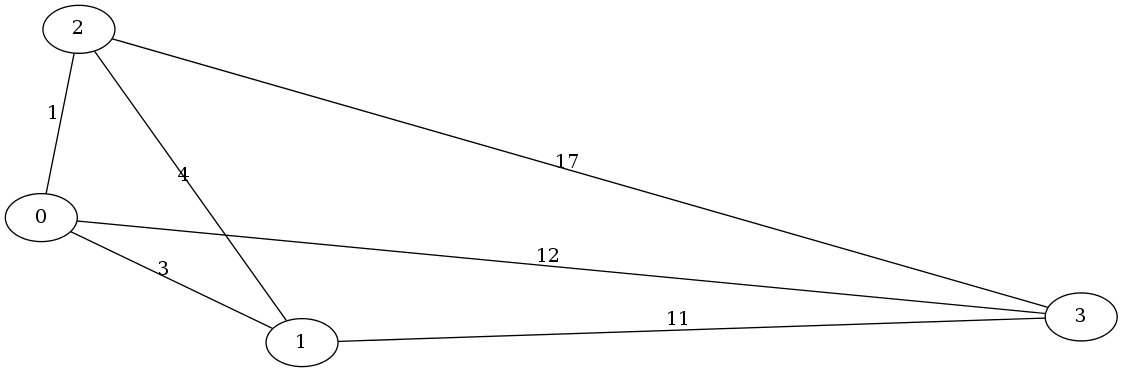
\includegraphics[width=1.0\textwidth]{good.png}
  \caption[width=0.8\textwidth]{Попарные расстояния в случае не сильно
    удалённых маркеров}
  \label{fig:fig1}
\end{figure}

На Рис. \ref{fig:fig2} показана идентичная ситуация для выборки из
четырёх маркеров, далеко расположенных друг от друга.

\begin{figure}[h]
 \centering
  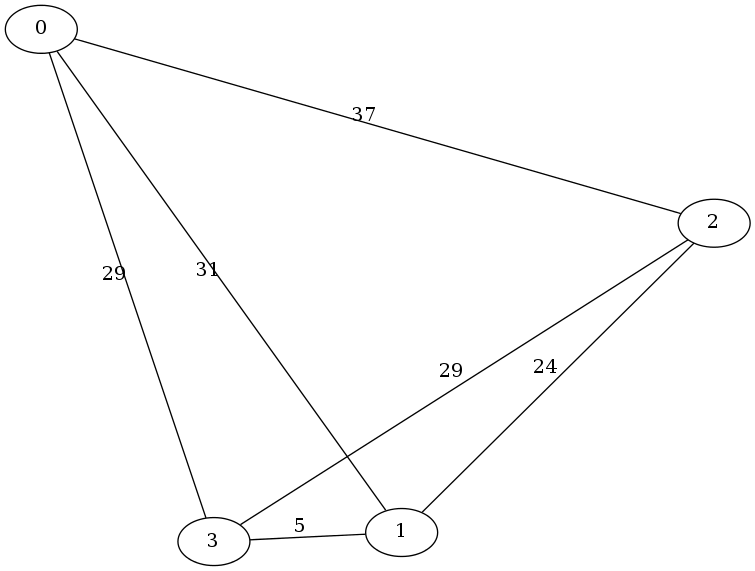
\includegraphics[width=0.7\textwidth]{bad.png}
  \caption[width=0.8\textwidth]{Попарные расстояния в случае сильно
    удалённых маркеров}
  \label{fig:fig2}
\end{figure}

Таким образом мы показали, что матрица частот рекомбинации является
оценкой матрицы попарных расстояний, причём оценка наиболее точна в
точках, находящихся близко друг к другу.

Исходя из приведённого выше замечания, мы считаем, что наиболее
правдивыми данными в матрице являются пары маркеров, с минимальными
значениями частоты рекомбинаций между ними, поэтому начинаем строить
карту от центра, представимого двумя самыми близкими маркерами. Более
формально этот алгоритм можно записать следующим образом:
\begin{enumerate}
\item Положим $n := dim(distMatrix)$
\item Выбираем из всех пар $(l,r)$ такую, что
  $distMatrix[l][r]$ был минимальным элементом матрицы
\item Положим массив $order := [l, r]$
\item Убираем $r$ и $l$ из просматриваемых узлов
\item Пока есть не рассмотренные узлы:
  \begin{enumerate}
  \item Положим $l = order[0]$
  \item Положим $r = order[-1]$
  \item Выбираем из оставшихся узлов такой узел $m$, который
    ближе всех к $l$ или $r$
  \item Убираем его из множества рассматриваемых узлов
  \item Если $m$ ближе к $r$:
    \begin{enumerate}
    \item Присоединяем к $order$ $[m]$ справа
    \item Присоединяем $[m]$ к $order$ слева
    \end{enumerate}
  \end{enumerate}
  \item Возвращаем $order$
\end{enumerate}
--- где входным параметром $distMatrix$ является квадратная матрица
частот рекомбинаций.

Применяя данный алгоритм, получаем результат в виде порядка маркеров.
На Рис. \ref{fig:fig3} видно, хоть представление и не линейно, что
есть некоторые ошибки, и что ошибки это порядка допустимых
транспозиций.
\begin{figure}[h]
 \centering
  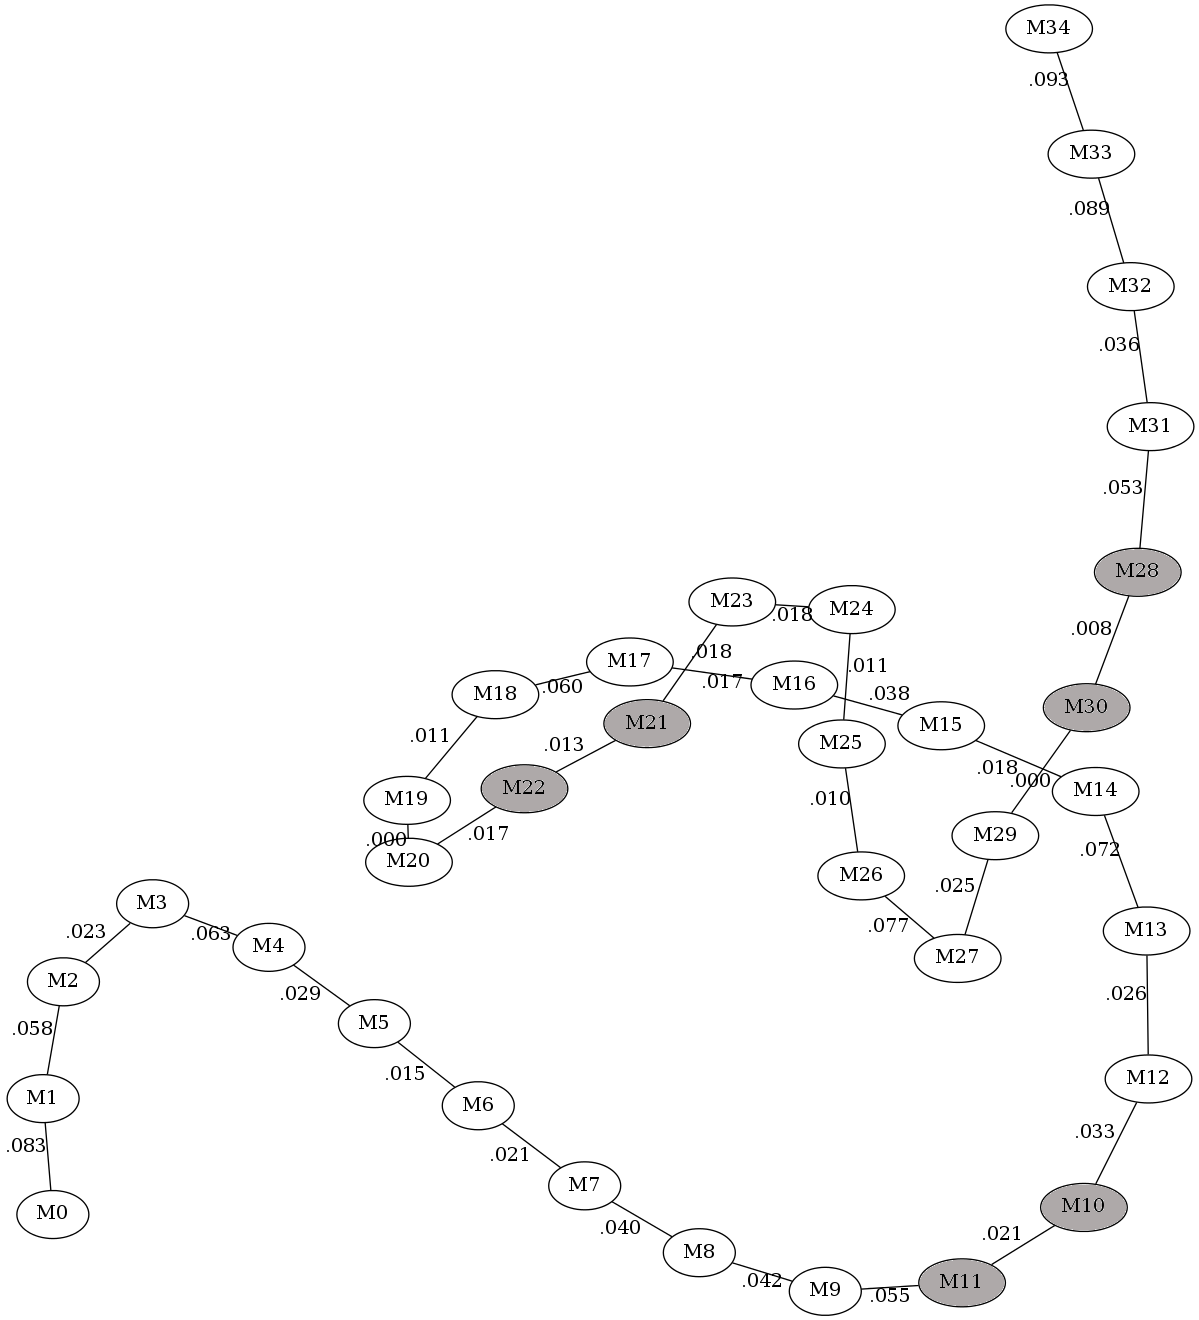
\includegraphics[width=0.85\textwidth]{linear.png}
  \caption[width=0.8\textwidth]{Порядок маркеров после применения
    алгоритма вытягивания в линию на семействе из 192 кошек с 35 маркерами}
  \label{fig:fig3}
\end{figure}
Посмотрев на рисунок можно попробовать представить изначальную матрицу
расстояний в виде графа с вершинами в маркерах и рёбрами с весами,
равными частоте рекомбинаций медлу двумя вершинами. Если вспомнить
алгоритм построения минимального остовного дерева Прима
\cite{cormen2001introduction}, который основывается на выборе ребра с
минимальным весом, что в нашем случае эквивалентно выбору пары
маркеров с минимальным расстоянием между ними среди всех остальных
пар, то логичным является попробовать находить порядок маркеров с
помощью алгоритма Прима. Заметим так же, что в случае правильно
построенной матрицы попарных расстояний, минимальным основным деревом
будет являться искомый порядок, который превратится в линию.
\begin{figure}[h]
  \centering
  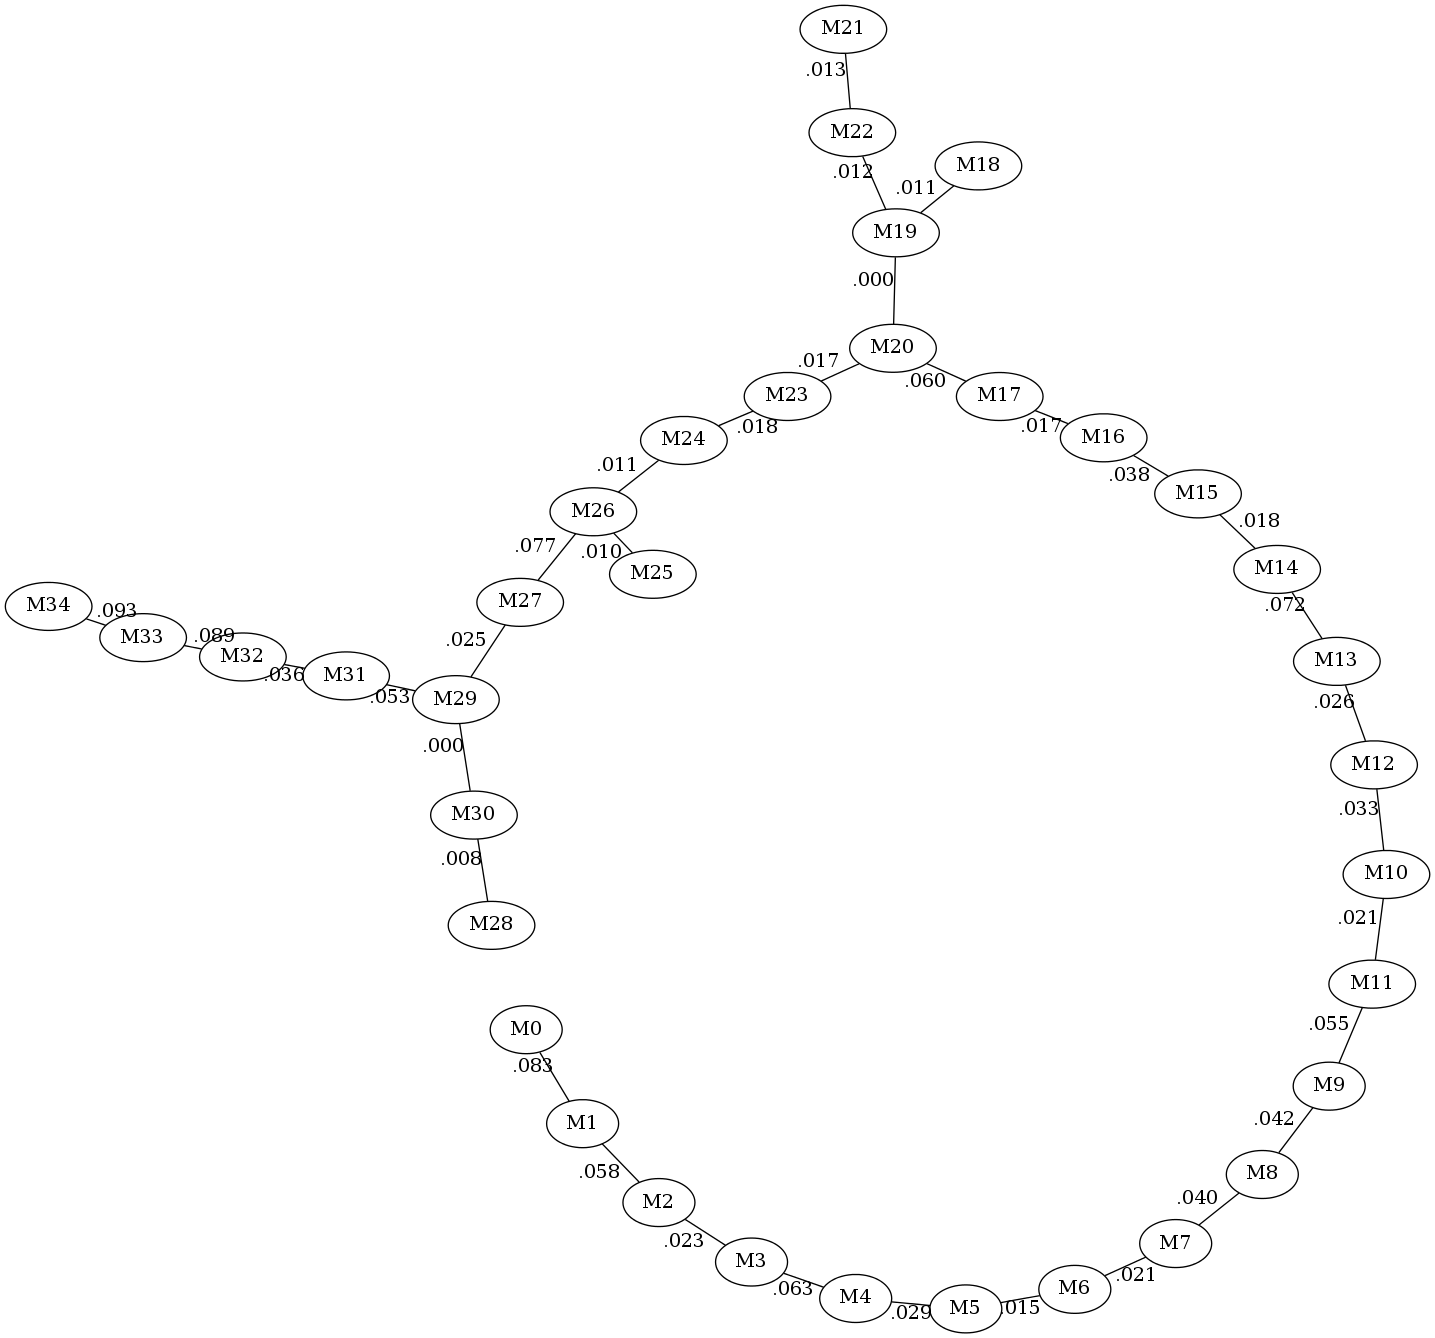
\includegraphics[width=0.85\textwidth]{prm.png}
  \caption[width=0.8\textwidth]{Минимальное остовное дерево графа
    попарных расстояний}
  \label{fig:fig4}
\end{figure}
На Рис. \ref{fig:fig4} представлено построенное с помощью алгоритма
Прима минимальное остовное дерево. Не трудно заметить, что те участки,
что не имели большого числа особенностей в первом варианте остались
неизменными, но появились особенности, которые не дают полученному
графу называться линией и упорядочить вершины, и если мы обратим
внимание на то, в каких вершинах проявляются особенности, то заметим,
что эти вершины либо не имеют данных о расстоянии с одним из соседей
(.000 на графе), либо проявляется в тех же местах, где нарушается
порядок в результатах первого алгоритма.

Данный пример показал, что в таких задачах применимы основы теории
графов и предположения о наибольшем правдоподобии маленьких
расстояний. Кроме того, показанный алгоритм при правильной организации
хранения графа имеет вычислительную сложность $O(M^2*log(M))$, что
вносит небольшое улучшение в алгоритм, так как в изначальной версии
алгоритма сложность $O(M^3)$. Воспользоваться алгоритмом Прима мы
сможем в случае, когда матрица частот рекомбинаций наиболее точно
приближает матрицу попарных расстояний.

\subsubsection{Повышение точности матрицы частот рекомбинаций}

Рассмотренные выше локальные оптимизации базируются на том, что
матрица попарных расстояний, полученная в результате извлечения
информации о происхождении аллели правдоподобна. Мы уже показывали,
что для далеко отстающих друг от друга маркеров оценка не верна.

Не трудно заметить, что точность получаемого результата зависит от
точности матрицы частот рекомбинаций, так как в нашем случае, именно
эта матрица является приближением матрицы попарных расстояний.  Как
было неоднократно замечено выше, алгоритм, на базе которого мы
пытаемся получить новое решение, не учитывает кратность кроссинговера,
в связи с чем, матрица частот рекомбинации актуальна только в случае
однократного кроссинговера. Резонной является задача извлечения данных
о кратных рекомбинациях, так как это явление случается в природе
достаточно часто.

Давайте попробуем рассмотреть функцию $f(d):\mathbb{R} \to \mathbb{N}$
--- функцию от расстояния между маркерами, возвращающую количество
произошедших рекомбинаций. Про эту функцию мы можем смело сказать, что
она неубывающая, потому что если рекомбинация произошла на участке,
разделяющем два маркера, то на более большом участке рекомбинаций
возможно не меньше, чем уже произошли. Но у этой функции есть
существенная проблема: строя генетические карты мы решаем
противоположную задачу, и расстояния между маркерами нам не известны.

Заметим, что частичные сведения о порядке и расстояниях нам даёт один
проход алгоритма по родословной. Допустим, основная его часть
верна. Естественным образом встаёт вопрос о возможностях уточнения
полученного порядка.

Нами было выдвинуто предположение, что базируясь на полученном после
одного прохода результе, можно уточнить его рассматривая каждую особь
повторно, аккумулируя матрицу частот рекомбинаций, зная примерное
расстояние между маркерами.

\subsection{Доработанный алгоритм}



Доработанный алгоритм реализует описанную выше схему. В этой главе мы
покажем, что эта схема оптимальная и более быстрая, чем наиболее
популярные сейчас алгоритмы.

Во-первых, так как в алгоритм были внесены существенные изменения,
стоит проверить, как это не отразилось на его асимптотике и
трудоёмкости.

\section{Сравнение алгоритмов}

Сравнение существующих алгоритмов на синтетических данных является
важной задачей, так как это позволяет выявить немало полезной
информации, такой как наиболее подходящие случаи для использования,
вероятные ошибки, вычислительную сложность. Кроме того, данные можно
генерировать дл акцентирования внимания на исследуемой
проблеме. Например, в случае исследования поведения программы на
данных, полученных путём моделирования кратного
кроссинговера. Заметим, что подобную информацию трудно получить из
естественных результатах секвенирования. Кроме того, параметризация
генерируемых данных упрощает проверку результата работы алгоритма.

\subsection{Генерация тестовых данных}

Генерация тестовых данных в случае генетики является задачей,
требующей аккуратности, так как во время моделирования сгенерированные
тестовые данные могут потерять биологический смысл.  При решении
этой задачи нами было выявлено 2 принципиально разных подхода:

\begin{itemize}
\item генерирование данных по заданным параметрам
\item генерирование данных на основе известного результата
\end{itemize}

В первом случае, генерируя тестовое множество особей, нам необходимо
понимать, каким образом выглядит итоговая и желаемая генетическая
карта.Во втором, имея карту, легко сравнивать получаемые результаты
работы алгоритма. Этот подход заведомо сложнее, так как никто не
гарантирует биекцию между множествами входных данных и множеством
результатов работы алгоритма на этих входных данных.  В связи с этим
мы выбрали первый подход.

Входные параметры:
\begin{itemize}
\item количество особей-прародителей (N)
\item количество прямых потомков (детей) (F1)
\item количество поколений (gen\_count)
\item итоговое количество особей в родословной (common\_N)
\item вероятность рекомбинации при мейозе (rec\_prob)
\item количество рассматриваемых маркеров (markers\_count)
\end{itemize}

Особь в нашем случае, это объект класса Organism

// тут будет код и его описание в виде листинга

Алгоритм генерации родословной:
\begin{enumerate}
\item Создаём пустой список pedigree длины common\_N
\item Генерируем m идентификаторов для маркеров
\item На основании количества особей-прародителей N генерируем аллели
  с m маркерами и задаём особям уникальный идентификатор
\item $N / 2$ особям указываем мужской пол, а оставшимся женский
\item Записываем в массивы possible\_fathers и possible\_mothers
  мужские и женские особи соответственно
\item Пополняем pedigree получившимися N особями
\item Пока $F1 > 0$:
  \begin{enumerate}
  \item mother <- possible\_mothers[random() mod $N / 2$]
  \item father <- possible\_fathers[random() mod $N / 2$]

АЛИНА, ПРИДУМАЙ ЧИТАЕМЫЙ ПСЕВДОКОД, ЭТОТ ДАЖЕ СЕЙЧАС НЕ ОЧЕНЬ, А ТЫ
ЕЩЕ ДО ОБРАЗОВАНИЯ ГАМЕТ НЕ ДОШЛА

  \end{enumerate}

\end{enumerate}

\subsection{Процесс сравнения и анализа}

Для наиболее хорошего и полного сравнения алгоритмов стоит выделить
ряд биологических аспектов, влияющих на результаты работы алгоритмов:
\begin{itemize}
\item наличие большого количества неинформативных пар (много
  гомозиготных локусов)
\item наличие неоднократного кроссинговера
\item его чётность
\end{itemize}

Не стоит забывать, что немаловажным для скорости выполнения алгоритма
является порядок количества маркеров и мощность родословной.

В связи с этим рассмотрим сочетания биологических особенностей,
влияющих на качество результатов алгоритмов, с объёмом данных.

ТАБЛИЧКА

\subsection{Обобщённые данные}
% BEGIN RECEIVE ORGTBL datasets
\begin{tabular}{rlll}
\hline
организмы and маркеры & 30 & 40 & 50 \\
\hline
200 & o200m30 & o200m40 & o200m50 \\
300 & o300m30 & o300m40 & o300m50 \\
400 & o400m30 & o400m40 & o400m50 \\
\hline
\end{tabular}
% END RECEIVE ORGTBL datasets
\iffalse
#+ORGTBL: SEND datasets orgtbl-to-latex :splice nil :skip 0
|-----------------------+---------+---------+---------|
| организмы and маркеры | 30      | 40      | 50      |
|-----------------------+---------+---------+---------|
|                   200 | o200m30 | o200m40 | o200m50 |
|                   300 | o300m30 | o300m40 | o300m50 |
|                   400 | o400m30 | o400m40 | o400m50 |
|-----------------------+---------+---------+---------|

\fi
Другие данные:
\begin{description}
\item[nocross] 200 кошек 30 маркеров без кросинговеров
\item[singlecross] 200 кошек 30 маркеров без кратных кроссинговеров
\item[manycross] 200 кошек 30 маркеров и очень много кроссинговеров
\item[cats] 192 кошки блеать
\end{description}

% BEGIN RECEIVE ORGTBL perf
\begin{tabular}{lrrr}
\hline
 & сыс & expO & expm \\
\hline
nocross & 0 & 0 & 0 \\
singlecross & 0 & 0 & 0 \\
manycross & 10 & 2 & 3 \\
cats & 1 & 0 & 0 \\
\hline
\end{tabular}
% END RECEIVE ORGTBL perf

\iffalse
#+ORGTBL: SEND perf orgtbl-to-latex :splice nil :skip 0
|-------------+-----+------+------|
|             | сыс | expO | expm |
|-------------+-----+------+------|
| nocross     |   0 |    0 |    0 |
| singlecross |   0 |    0 |    0 |
| manycross   |  10 |    2 |    3 |
| cats        |   1 |    0 |    0 |
|-------------+-----+------+------|
\fi

% BEGIN RECEIVE ORGTBL qual
\begin{tabular}{llll}
\hline
 & сыс & expO & expm \\
\hline
o200m30 & 1c & 10m & 1h \\
o200m40 & 1c & 10m & 2d \\
o200m50 & 2c & 10m & $\infty$ \\
o300m30 & 2c & 1d & 2h \\
o300m40 & 3c & 1d & 2d \\
o300m50 & 3c & 1d & $\infty$ \\
o400m30 & 5c & $\infty$ & 3h \\
o400m40 & 6c & $\infty$ & 3d \\
o400m50 & 8c & $\infty$ & $\infty$ \\
\hline
\end{tabular}
% END RECEIVE ORGTBL qual
\iffalse
#+ORGTBL: SEND qual orgtbl-to-latex :splice nil :skip 0
|---------+-----+----------+----------|
|         | сыс | expO     | expm     |
|---------+-----+----------+----------|
| o200m30 | 1c  | 10m      | 1h       |
| o200m40 | 1c  | 10m      | 2d       |
| o200m50 | 2c  | 10m      | $\infty$ |
| o300m30 | 2c  | 1d       | 2h       |
| o300m40 | 3c  | 1d       | 2d       |
| o300m50 | 3c  | 1d       | $\infty$ |
| o400m30 | 5c  | $\infty$ | 3h       |
| o400m40 | 6c  | $\infty$ | 3d       |
| o400m50 | 8c  | $\infty$ | $\infty$ |
|---------+-----+----------+----------|
\fi


\section*{Заключение}

\subsection*{Результаты}

В ходе выполнения дипломной работы нами был предложен доработанный
алгоритм прямого извлечения информации о рекомбинациях из
секвенированного генома, позволяющий получать генетические карты в
случае одно- и многократного кроссинговера.  Для верификации нового
алгоритма был реализован механизм тестирования методов построения
генетических карт, с помощью которого были наглядно представлены
преимущества нашей реализации алгоритма.

\subsection*{Актуальность полученных результатов}

Применение генетических карт получило достаточно широкое
распространение в сфере диагностирования наследственных
заболеваний. Исследование механизмов наследования, а так же выявление
его закономерностей позволяет получить информацию о
предрасположенности у человека (и не только) к тем или иным
отклонениям, которые трудно выявить до начала проявления
симптомов. Получение информации о генной предрасположенности до начала
заболевания позволяет моделировать лечения и образ жизни, избегая или
купируя их дальнейшие проявления.

Кроме того, генетические карты применяются в исследованиях процессов
эволюции. Рассматривая генетические карты двух достаточно близких
видов, можно извлечь информацию о том, в каком направлении
эволюционировала фауна и какие гены передавались в первую очередь.

Из-за недостатков современных методов секвенирования, а так же из-за
отсутствия возможности секвенировать гаметы, единственными способами
построить генетическую карту являются рассмотренные выше
алгоритмы. Предложенный нами алгоритм позволяет строить карты быстрее,
чем альтернативные алгоритмы, и точнее, чем его предшественник.

\bibliographystyle{unsrt}
\bibliography{diploma.bib}
\end{document}
